%
%   N K Y M
%    A A A A
%

%   this file is "nkym.tex"

\documentclass[10pt,b5paper,papersize,dvipdfmx]{jsbook}

\usepackage[analog]{vuccaken}
\usepackage{v-hyperref}
\usepackage{vuccaken2019}

\usepackage{newtxtext,newtxmath}

%% font -> gt & sf
\renewcommand\kanjifamilydefault{\gtdefault}
\renewcommand\familydefault{\sfdefault}

%% メモ
%% 証明の環境作る

\begin{document} % - - - - - - - - - - - - - - - - - - - - - -

\newcommand\karizu[1]{\begin{center}(図:#1)\end{center}}

\newif\ifsecI
\newif\ifsecII

\secItrue
\secIItrue

\mokuji{2}

% - - - - - - - - - - - - - - - - - - - - - - - - %
\kaishititle%
  {私、実在の記述は完全でって言ったよね!}% title
  {物理科学科4回生}% 所属
  {中山~敦貴}% name
% - - - - - - - - - - - - - - - - - - - - - - - - %

% \IfFileExists{enumitem.sty}{exist}{not exist}

% - - - - - - - - - - - - - - - - - - - - - - - - %
\section*{はじめに}
% - - - - - - - - - - - - - - - - - - - - - - - - %
とりあえず、内容としましては、古典力学で仮定されていた局所実在論では説明できないようなことが量子の世界では起こっているという話をします。
具体的には、局所実在論であれば必ず成立するベルの不等式が、エンタングルメントという量子論特有の性質を持った系では破れることがあるということを示します。\par
章立ては大きくは以下のような感じだと思います。


\ifsecI
% - - - - - - - - - - - - - - - - - - - - - - - - %
\section{実在論と量子論}
% - - - - - - - - - - - - - - - - - - - - - - - - %

%
\subsection{局所実在論} % - - - - - - - - - - -

ここでは「局所実在論」という立場について説明する。
\par
まず、普通の人が持っている「世界は見たままに存在している」という世界観を「\ftj{素朴実在論}」と呼ぶことにしよう。
例えば、「誰も見ていなくても、月は存在している」や「猫は生きているか死んでいるかのどちらかである」のような、モノや状態の実在についての考え方である。
当たり前のことすぎるかもしれないが、古典力学\footnote{
  これから話す相対性理論も古典力学の一種である。古典力学でないものは量子力学と呼ばれる。
}はそういう立場にあるということだけ覚えておいてほしい。
\par
また、古典力学の最終形態である相対論から、\ftj{局所性}という要請がなされる。
局所性とは、「空間的に離れた2点間において、何物も光速を超えて伝わることはない」という要請である\footnote{
  ニュートン力学では重力などの力は一瞬で伝わるものとされていたが、相対論では力であれ何であれ光速度を超えて伝わることはないとされる。
}。これが意味することは、遠く離れた2つの系を考えるとき、ごくわずかな時間であれば独立な系として扱ってよいということである。
詳しくは述べないが、この局所性という要請は、「因果律」を守る\footnote{
  すなわち、ある2つの事象(event)について、どの慣性系で見てもどちらが先に起きてどちらが後に起きたかは一意的に決まるということ。
}ための条件として、物理の理論には必要とされるものである。
\par
以上のことから、我々は、素朴実在論に局所性を加えた「\ftj{局所実在論}」という立場をとることにしよう。
局所実在論とはすなわち、因果律を守るような古典論ということである。
そして、アインシュタインもこの立場であった。

\karizu{光円錐}

%
\subsection{EPR論文} % - - - - - - - - - - -
%

20世期初頭、アインシュタインの特殊相対性理論の発表に少し遅れて、量子力学が成立した。
この量子力学というものからは、これまでの常識を根本から覆すような予測がいくつもなされたが、それらは実験によって確かに正しいということが確認されていった\footnote{
  検証実験の繰り返しによって理論の正しさを推論するのは帰納法であるから、何度検証を行おうが理論が$100\tani{\%}$正しいと推論することはできない。
  ただし、もし検証結果が理論の予測と異なる場合に、その理論は正しくないと推論することは演繹法であるから、その理論は$100\tani{\%}$正しくないと断言できる。\par
  科学におけける推論では演繹法だけでなく、帰納法も用いられているため、一般には絶対的に正しいという推論はできない。しかしこの演繹と帰納の絶妙なバランスこそが、今日の目覚ましい科学の発展の要因のひとつであろうかと思う。
}。
\par
そんな中、1935年5月にアインシュタイン・ポドルスキー・ローゼンらは、「量子力学は実在の記述に関して完全でない」という主張の論文を発表した。
のちにEPRパラドックス\footnote{
  実際は、この論文にパラドックス(矛盾)はない。
}などと呼ばれるようになるこの論文の内容について、これから詳しく見ていく。

%
\subsubsection{EPR論証(思考実験)} % - - - - - - - - - - -

EPR論文では、まず次の2つを前提としている:
\begin{enumerate}[{label=[\arabic*]}]
  \item 完全な理論においては、実在の要素のそれぞれに対する要素が存在する。\label{enm:z1}
  \item 系を乱さずに値を確率1で予測できる物理量には、それに対応する実在の要素が存在する。\label{enm:z2}
\end{enumerate}
\par
前提\ref{enm:z1}では、完全な理論がどういうものかを定義している。
例えば、完全な理論では、もしある電子の運動量が実在するならば、その運動量の測定値を予測できるようなものでなければならない。\par
前提\ref{enm:z2}では、物理量が実在するとはどういうこのなのかを定義している。
例えば、ある電子の運動量の測定値が、ある時刻にはいくらであるかを、その電子にはなんら影響を与えずに予測できるなら、その電子の運動量は\ftj{実在する}と言える。
\par
これらの前提を踏まえた上で論証を行う。
初めに、次の2つの仮定をする:
\begin{itemize}
  \item 2つの電子I, IIがあり、これらの「位置の差」と「運動量の和」は分かっているとする。
  \item 電子IとIIは、互いに空間的に離れているので、電子Iに対する測定が一瞬で電子IIの状態に影響を与えることはない。
\end{itemize}

ハイゼンベルクの不確定性原理として知られているように、一般に非可換な物理量\footnote{
  量子力学では、物理量と測定値の概念は区別される。物理量はエルミートな演算子(行列)であり、測定値はその固有値(ただの数)とされる。
  線形代数で習ったように、行列は一般には非可換であるから、物理量も一般には非可換である。
}に同時に決まった値を持たせることはできない(同時固有状態は存在しない)。
しかし、「位置の差」と「運動量の和」の交換関係を調べてみると
\begin{align*}
  \comm{\hat r_I - \hat r_{II}}{\hat p_I + \hat p_{II}}
  &= \comm{\hat r_I}{\hat p_I} + \comm{\hat r_I}{\hat p_{II}} - \comm{\hat r_{II}}{\hat p_I} - \comm{\hat r_{II}}{\hat p_{II}} \\
  &= i\hbar + 0 - i\hbar - 0
  = 0
\end{align*}
となるので、2つの電子I, IIの「位置の差」と「運動量の和」が同時に分かっているという状況(同時固有状態)はあり得る。
よって、1つ目の仮定は量子力学に反していない。
また、2つ目の仮定は、前のセクションで述べた局所実在論という立場によるものである。\par
すると、2つの電子I, IIの「位置の差」が分かっているので、電子Iの位置を測定することで、電子IIの系を乱すことなく、電子IIの位置も測定することができるはずである。
また、運動量についても同様である。\par
ここで、前提\ref{enm:z2}より、電子IIの位置と運動量はともに実在の要素であると言える。\par
ところが、電子IIの位置と運動量は非可換な物理量であるから、位置と運動量の同時固有状態は存在しない。
すなわち、量子力学の理論では、電子の位置と運動量という実在の要素に対して、それらに対応する要素(固有状態)を同時に用意することはできない。\par
よって、前提\ref{enm:z1}より、量子力学は完全な理論でないと結論づけられる。

%
\subsubsection{EPR論証に対する反応} % - - - - - - - - - - -

ここで行った論証は、経験を認めると、量子力学という理論は、実在の記述に関しては完全でないという主張を示したものであって、決して量子力学が間違っているといったものではない。
さらに言えば、「完全な理論」や「実在」という概念も上で定義した意味で用いているのであって、この定義が妥当かどうかにも議論の余地がある。\par
物理量の実在に関して、ボーアは「どの物理量が実在するかは実験の状況に依存する」という意見を持っていた。
すなわち、電子の位置を測定するときには確かに電子の位置は実在しているが、この状況においては電子の運動量は実在していないということである。
このように、どの物理量を測定するかによって、どの物理量が実在するか変わってしまうというボーアの解釈は、今日では様相解釈の一種とされる。\par
これに対し、アインシュタインらは、もしEPR論文での実在の定義が妥当でないにしても、どのような実験をするかによって物理量の実在性が決まるといった議論は認められないとしている。
そのようなものは、もはや実在とは呼べないということであろう。\par
また、現在では電子IとIIの間に非局所的な相関があったと解釈するのが主流である(コペンハーゲン解釈)。
この解釈の相対論との整合性は、最後のセクションで説明することにする。\par
EPR論文が発表された当時は、このような議論は形而上学の問題\footnote{
  反証可能性のないただの哲学の問題であって、どのような解釈をしようが結果は同じということ。それに対し、物理学は形而下学とも呼ばれる。
}であるとされ、多くの物理学者からは無視されていた。
また、物理量に実在を持たせるため、既存の量子力学に代わるようなものとして、隠れた変数理論\footnote{
  既存の量子力学では、系の時間発展が一般には確率的にしか予測できないということ(射影公準)は公理に含まれているが、この性質は統計的なものであって、本当は未だ観測されていない隠れた変数が存在し、それによって系の時間発展は決定論的に予測できるとする理論。
}というものがいくつか提案された。
しかし、どれも既存の量子力学と同じ予測能力しかなく、やはりこれもただの解釈問題とされてきた。\par
このような状況の中、1964年にベルはある論文を発表する。
それは、「局所的な隠れた変数理論であれば、ある不等式(ベルの不等式)を必ず満たすが、(既存の)量子力学で考えるとこの不等式を満たさない場合がある」ということを示すものであった。
すなわち、局所的な隠れた変数理論(局所実在論)と量子力学では異なる予測をするということが分かったのである。
このことは、自然を正しく記述する局所的な隠れた変数理論が存在するか否かを、実験で(科学的に)検証できるということを意味する! \par
その後、アスぺによる検証が行われ、自然は量子力学の予想通りベルの不等式を破ることが実証された。
それによって、自然を正しく記述することができる局所的な隠れた変数理論は存在しないということが示された。
すなわち、どんな局所実在論を作ったとしても、それで自然を正しく記述することはできない。それができるのは、(今のところ)量子力学だけである\footnote{
  自然を正しく記述できる局所実在論が存在しないという推論は、演繹法であるから$100\tani{\%}$正しい。
  しかし、そのことは量子力学の正しさを論理的に保証するものではない。
  この検証によって量子力学は生き残っただけであり、その正しさが増したと主張する根拠は論理的には全くない。
  とはいえ、感覚的には確かに量子力学の信頼性は向上したように思える。
}。\par
このベルの不等式とアスペの実験については、これから詳しく見ていく。

\fi
\ifsecII
% - - - - - - - - - - - - - - - - - - - - - - - - %
\section{ベルの不等式}
% - - - - - - - - - - - - - - - - - - - - - - - - %

このセクションでは、局所的な隠れた変数理論あれば必ずベルの不等式を満たすことを証明する。
さらに、量子力学の理論で考えると、ベルの不等式を破る場合があることを示す。
のちに、アスペによる検証で、実験的にベルの不等式が破れる場合があることを認めざるを得なくなる。
もちろん、物理学は実験科学であるから、経験を否定することはできない\footnote{
  量子力学が正しくないという主張は別に構わないが(とはいえ反証可能性は必要だが)、経験(実験事実)は正しいと認めなければならない。
}。\par
まずは、局所的な隠れた変数理論において、ベルの不等式が成り立つことを示そう。

%
\subsection{ベルの不等式} % - - - - - - - - - - -

ベルの不等式(ベル型の不等式)にはいくつか種類があるが、ここではベルのオリジナルのものではなく、CHSH\footnote{
  John Clauser, Michael Horne, Abner Shimony, and Richard Holt (1969).
}不等式と呼ばれるものを示すことにする。


%
\subsubsection{不等式の証明}
\hyo{pm}のように$x, \theta, \phi$の3列に$+, -$を好きに割り振るゲームを考える。
この表の中で$x$と$\phi$にそれぞれ$+$があるものの個数を$n(x=+,\phi=+)$のように書くと、次の不等式が必ず成り立つ:
\begin{align}
  n(x=+,\phi=+) + n(\phi=-,\theta=+) \ge n(x=+,\theta=+).
  \label{eq:bell's ineq}
\end{align}

\begin{table}[htbp]
  \centering
  \caption{$+, -$の割り振り}
  \label{tab:pm}
  \begin{tabular}{ccc} \hline
    $x$ & $\theta$ & $\phi$ \\ \hline
    $+$ & $+$ & $-$ \\
    $-$ & $+$ & $+$ \\
    $-$ & $-$ & $-$ \\
    $+$ & $+$ & $-$ \\
    $+$ & $-$ & $+$ \\
    $\vdots$ & $\vdots$ & $\vdots$ \\ \hline
  \end{tabular}
\end{table}

\noindent 証明:\par
\hyo{pm}において$n(x=+,\phi=+)$は、$\theta = +$の場合と$\theta = -$の場合の和で書けるはずである\footnote{
  $n(x=+,\phi=+)$と書いたとき、隠れた変数である$\theta$の値については何も言及されていない。
  実在論の立場では、たとえ隠れていようが、$\theta$は必ずある値($+$か$-$のどちらか一方)を持っているものとする。
}。すなわち
\begin{align}
  \label{eq:bell-1}
  n(x=+,\phi=+) = \textcolor{red}{n(x=+,\phi=+, \theta=+)} + n(x=+,\phi=+, \theta=-).
\end{align}
同様にして
\begin{align}
  \label{eq:bell-2}
  n(\phi=-,\theta=+) &= \textcolor{blue}{n(x=+, \phi=-,\theta=+)} + n(x=-, \phi=-,\theta=+)
  , \\
  \label{eq:bell-3}
  n(x=+,\theta=+) &= \textcolor{red}{n(x=+, \phi=+, \theta=+)} + \textcolor{blue}{n(x=+, \phi=-, \theta=+)}.
\end{align}
\siki{bell-1}と\siki{bell-2}の和と\siki{bell-3}を比較すると、\siki{bell-1}と\siki{bell-2}の第2項の分だけ\siki{bell-3}の方が小さい。よって、ベルの不等式\siki{bell's ineq}が成り立つ。
\QED

%
\subsection{アスペの実験} % - - - - - - - - - - -
Ca原子から放出される2つの光子を検出する実験を考える。
すると、量子論から予想される値を用いたのでは、ベルの不等式が破れてしまう場合があることが導かれてしまう。
自然をより正しく記述するのは局所実在論か量子論か、それらは実験によって判断される。
そして、アスペによる検証で、後者が正しいことが示された。\par
このことについて詳しく見ていく。
まずは、光子の性質から確認していこう。

%
\subsubsection{光子の偏光} % - - - - - - - - - - -

光子の電場の振動の方向を、光子の偏光と呼ぶ\footnote{
  光子は粒子だが、波動としての性質(偏光)も同時に持っている。
}。
光子の進行方向、電場(偏光)および磁場の方向は、それぞれ互いに直交している。

\begin{figure}[ht]
  \centering
  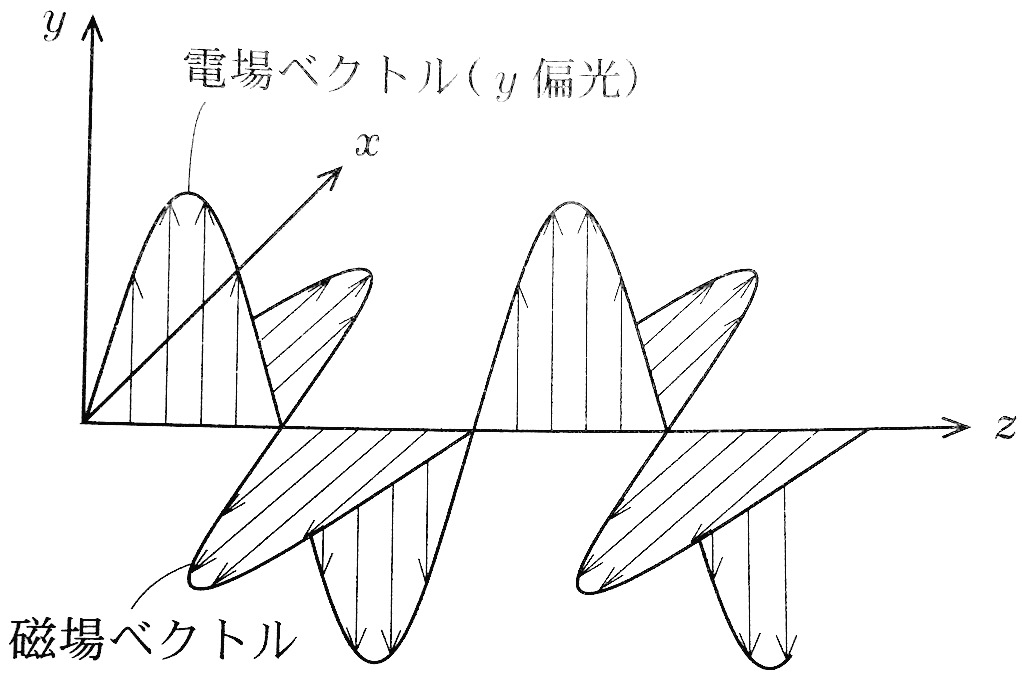
\includegraphics[width=40mm]{nkym/fig/henkou.jpeg}
  % \caption{軸の設定。(参考文献[1], P.26)}
  % \label{}
\end{figure}

\par
また、偏光子\footnote{
  サングラスとかに使われる偏光板のようなものだと思えば良い。
}と呼ばれるものが存在し、次のような性質を持つ\footnote{
  理論的な証明は面倒なので、実験事実(経験)としてこれらの性質を認めていただきたい。
  何度も言うが、物理学は実験科学なので、実験事実(経験)こそが正しさの絶対的基準である。
}:
\begin{itemize}
  \item 偏光子を通過した後の光子の偏光は、偏光子の偏光軸と一致する。
  \item 光子が偏光子を通過する確率は、光子と偏光子の偏光軸のなす角を$\theta$とすると
    \begin{align}
      P(\theta) = \frac12 \cos^2\theta
    \end{align}
    である。
\end{itemize}

%
\subsubsection{Ca原子の放射光の検出} % - - - - - - - - - - -

Ca原子にレーザー光を照射して、特定のエネルギーレベルに励起させると、基底状態に戻る際に2個の互いに直交した偏光を持つ光子(緑色と紫色)が放出される\footnote{
  これについても、ここでは実験事実として認めていただきたい。
}。\par
以上を踏まえ、\zu{Ca-machine}のような装置で2つの光子を検出することを考える。

\begin{figure}[htb]
  \centering
  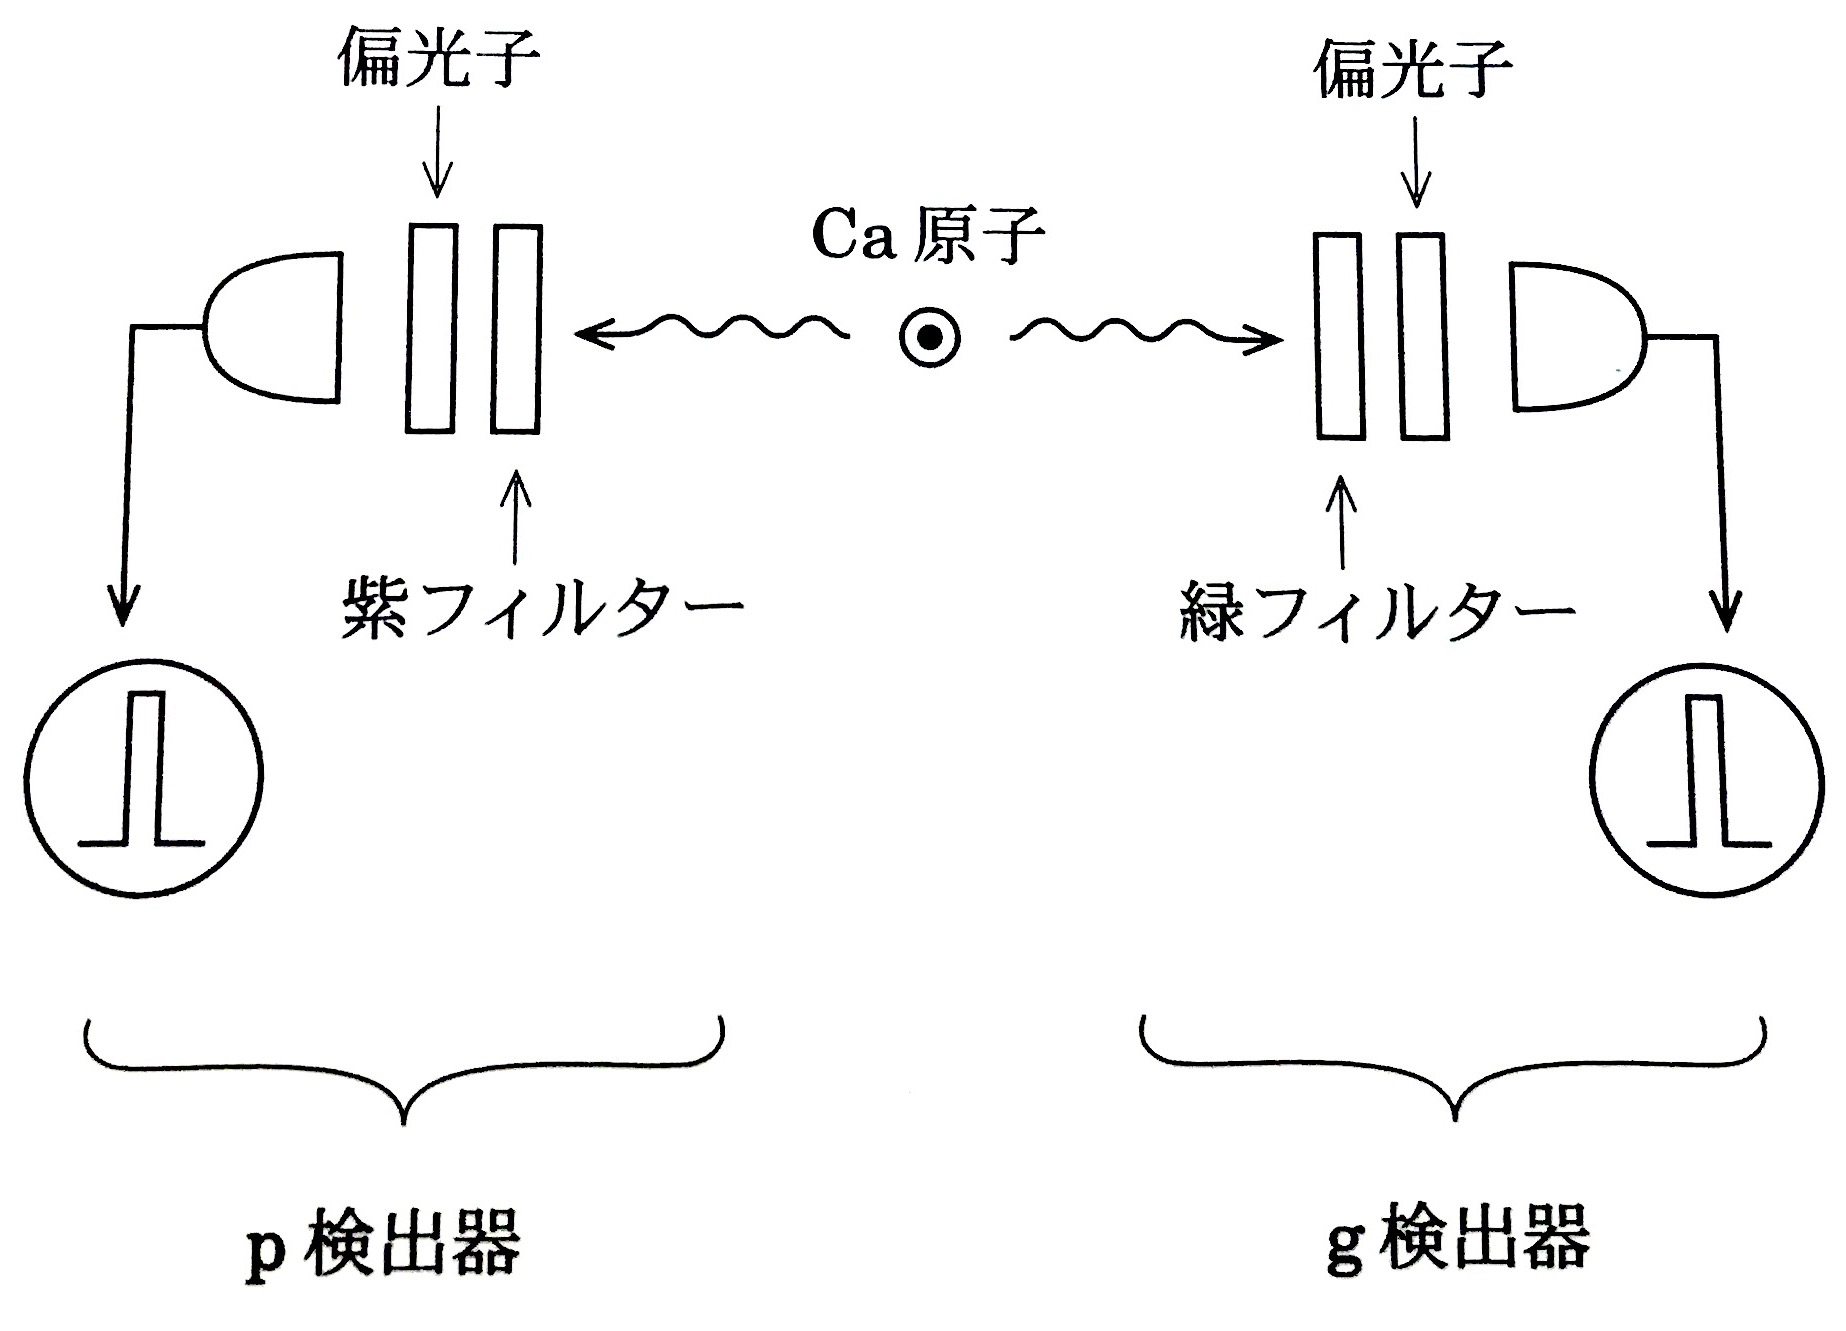
\includegraphics[height=40mm]{nkym/fig/souchi.jpeg}
  \caption{Ca原子から出た2つの光子の偏光を検出する装置。} %(参考文献[1], P.21)
  \label{fig:Ca-machine}
\end{figure}

%
\subsubsection{検出器の偏光軸} % - - - - - - - - - - -

\begin{figure}[ht]
  \centering
  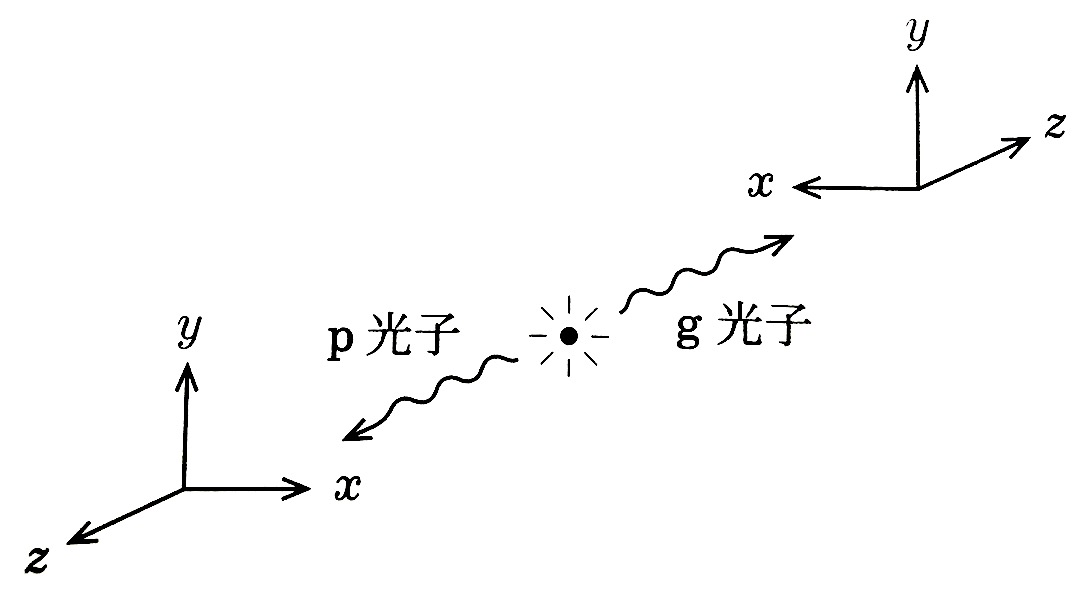
\includegraphics[width=40mm]{nkym/fig/zahyou-kei.jpeg}
  \caption{偏光を表すための座標軸の設定。} %(参考文献[1], P.26)
  \label{fig:zahyou-jiku}
\end{figure}

光子の進行方向を$z$軸正の向きとし、水平方向に$x$軸、鉛直方向に$y$軸をとる\footnote{
  実験系に固定した座標系を取るのではなく、光子それぞれに対して座標系を取ることに注意。
  % 例えば、一方の光子の偏光が$x$軸であれば、
}。
p検出器とg検出器に付いている偏光子の偏光軸は、\zu{henkou-jiku}のように、それぞれ2種類の設定を使う。

\begin{figure}[ht]
  \centering
  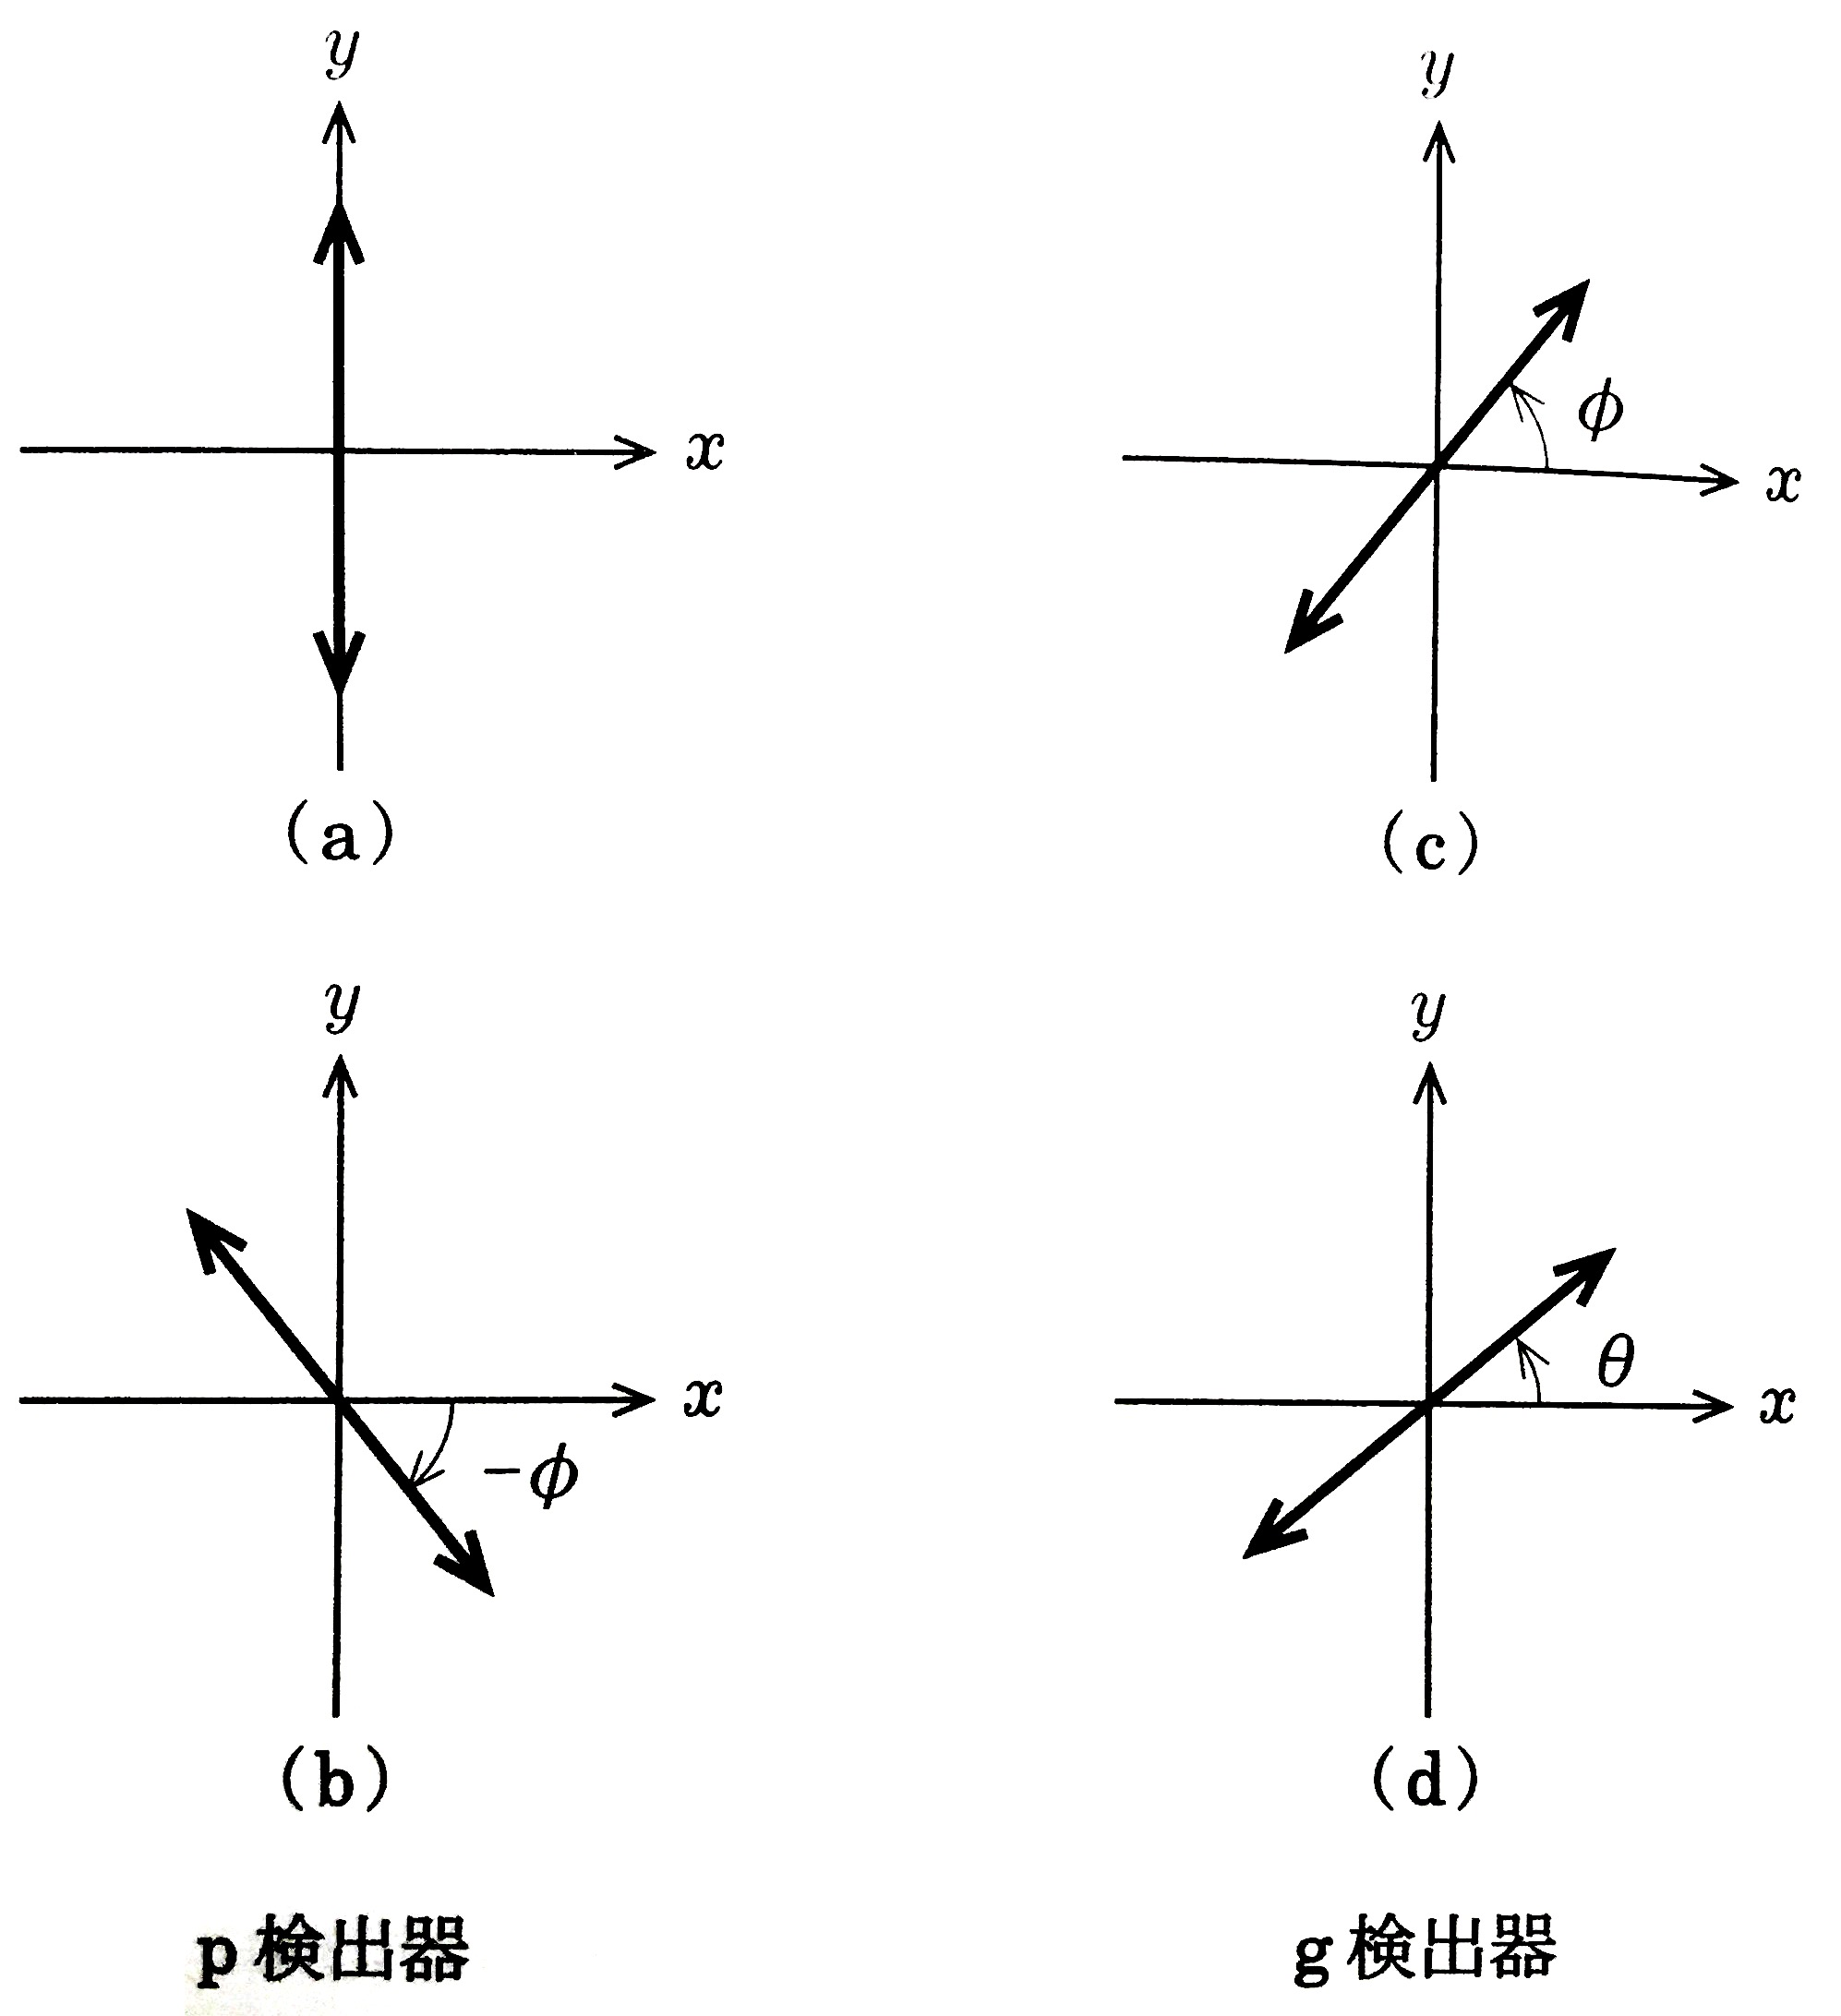
\includegraphics[width=45mm]{nkym/fig/henkou-jiku.jpeg}
  \caption{偏光子の偏光軸の方向。} %(参考文献[1], P.26)
  \label{fig:henkou-jiku}
\end{figure}

%
\subsubsection{光子の測定} % - - - - - - - - - - -

p検出器の偏光子の偏光軸を$y$軸方向に、g検出器の偏光軸を$x$軸から$\phi$だけ回してセットし、単位時間あたりに両検出器が同時に光子を検出する回数$n(x=+,\phi=+)$を観測する。
同様にして、$n(x=+,\theta=+)$と$n(\phi=-,\theta=+)$を観測する。\par
単位時間当たりにp検出器が検出する光子の数を$N \,(\gg 1)$個として、同時にg検出器が光子を検出する数を予想すると、次のようになる:
\begin{align}
  \label{eq:photon-1} n(x=+,\phi=+)      &= N \cos^2\phi, \\
  \label{eq:photon-2} n(x=+,\theta=+)    &= N \cos^2\theta, \\
  \label{eq:photon-3} n(\phi=-,\theta=+) &= N \cos^2(\phi + \pi/2 - \theta) = N \sin^2(\phi - \theta).
\end{align}

%
\subsubsection{ベルの不等式の破れ} % - - - - - - - - - - -

上で示した\siki{photon-1}から\siki{photon-3}を、ベルの不等式\siki{bell's ineq}に代入すると、次のようになる:
\begin{align*}
  \cos^2\phi + \sin^2(\phi - \theta) \ge \cos^2\theta.
\end{align*}

ここで、$\phi = 3\theta$とし、右辺を左辺へ移項すると
\begin{align}
  \cos^2 3\theta + \sin^2 2\theta - \cos^2\theta \ge 0
\end{align}
となる。
しかし、左辺を$\theta$の関数として図示すると(\zu{left-hen})、$0 < \theta < 30^\circ$の範囲で不等式を満足しないことがわかる。

\begin{figure}[htp]
  \centering
  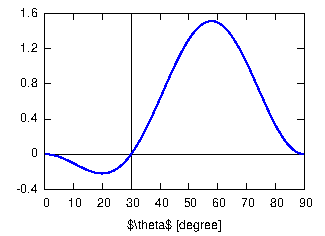
\includegraphics{nkym/fig/Aspect.pdf}
  \caption{不等式の左辺。}
  \label{fig:left-hen}
\end{figure}

ここで、局所実在論と量子論との間で矛盾が生じている。
果たして、どちらの理論が正しいのであろうか?

初めにも述べたとおり、結局、アスペらによる検証実験によって、量子論の予想通りベルの不等式を満たさない場合があることが示された。
さらに、実験によって得られた値は、量子論で予想された値とピタリと一致した\footnote{
  もちろん、エラーバーはあるが、標準偏差は不等式の破れに比べて何倍も小さいものであったらしい[要出典]。
}。
この実験結果は、自然を正しく記述できる局所実在論(隠れた変数理論)の存在を否定するだけでなく、量子論の正しさを保証する積極的な根拠であるとも言える。

\subsection{解釈}

最後に、以上の結果はどのように解釈されるのかを述べる。

\begin{itemize}
  \item 例えば$n(x=+,\phi=+)$を測定したとき、$\theta$が何であったかには言及していない(測定していない)。
  \item ベルの不等式を導く際は、$\theta$は隠れているだけで、$\theta=+$か$\theta=-$の事象が起きたはずだと仮定していた。
  \item 実はこの仮定が間違っており、3列に$+,-$を割り振るゲームと、アスぺの実験で考えた状況は異なるものであった。
\end{itemize}

つまり

\begin{itemize}
  \item 測定していない物理量は、常に確定(実在)しているとは限らない。
  \item アスぺの実験では、Ca原子から放出される2つの光子の偏光が互いに直交しているということがポイント。(エンタングルメント)
\end{itemize}

まとめ

\begin{itemize}
  \item 隠れた変数(理論)があれば、必ずベルの不等式を満たす。
  \item 偏光軸が直交した2つの光子(エンタングル状態)を用いた実験では、ベルの不等式を満たさない場合があることがわかった(アスぺの実験)。
  \item この実験結果は、隠れた変数理論(実在論)では記述できないような現象があることを示唆している。
  \item 周知の通り、量子力学では上のような現象も問題なく予測できる。つまり、量子力学は古典論を含み、かつ実在論を超えた理論である。
\end{itemize}

\fi
% - - - - - - - - - - - - - - - - - - - - - - - - %
\section{まとめ?}
% - - - - - - - - - - - - - - - - - - - - - - - - %

\begin{itemize}
  \item まとめ
  \item 今後の展望
\end{itemize}

% \begin{figure}[htbp]
%   \centering
%   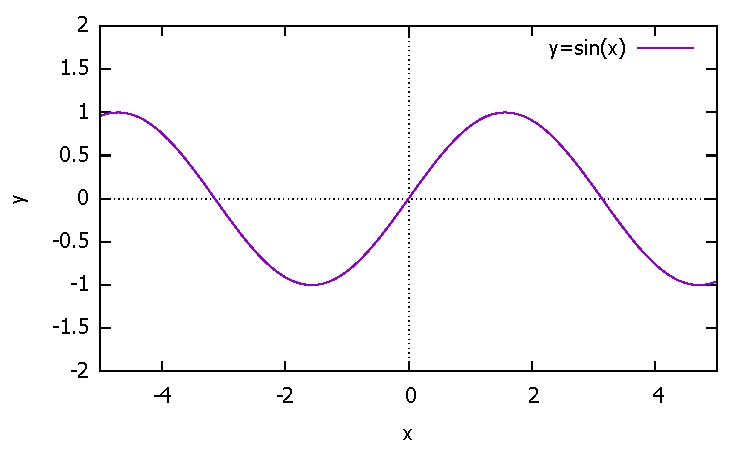
\includegraphics[width=10cm]{temp/fig-sin.pdf}
%   \caption{$y=\sin x$のグラフ。gnuplotで作成した。}
%   \label{fig:sin}
% \end{figure}



%% 参考文献
\begin{thebibliography}{99}
  \item 清水明、「新版 量子論の基礎」、サイエンス社、2004年。
  \item 清水明、スライド「EPRパラドックスからベルの不等式へ」\\
  \url{http://as2.c.u-tokyo.ac.jp/lecture_note/kstext04_ohp.pdf}
  \item J.J.サクライ、「現代の量子力学(上)」、吉岡書店。
  \item 森田邦久、「アインシュタイン vs. 量子力学」、化学同人。
  \item 森田邦久、「量子力学の哲学」、講談社現代新書。
  \item 荒船次郎 他、「現代物理学の歴史 I」、朝倉書店。
  \item 宮野健次郎、古澤明『量子コンピュータ入門』、日本評論社(2019)。
\end{thebibliography}


\end{document}
%
% EOF
%